\documentclass[
11pt, % The default document font size, options: 10pt, 11pt, 12pt
%codirector, % Uncomment to add a codirector to the title page
]{charter} 


% El títulos de la memoria, se usa en la carátula y se puede usar el cualquier lugar del documento con el comando \ttitle
\titulo{Sistema de alarmas para el mantenimiento de videocámaras} 

% Nombre del posgrado, se usa en la carátula y se puede usar el cualquier lugar del documento con el comando \degreename
%\posgrado{Carrera de Especialización en Sistemas Embebidos} 
%\posgrado{Carrera de Especialización en Internet de las Cosas} 
\posgrado{Carrera de Especialización en Inteligencia Artificial}
%\posgrado{Maestría en Sistemas Embebidos} 
%\posgrado{Maestría en Internet de las cosas}
% IMPORTANTE: no omitir titulaciones ni tildación en los nombres, también se recomienda escribir los nombres completos (tal cual los tienen en su documento)
% Tu nombre, se puede usar el cualquier lugar del documento con el comando \authorname
\autor{Ing. Marco Joel Isidro}

% El nombre del director y co-director, se puede usar el cualquier lugar del documento con el comando \supname y \cosupname y \pertesupname y \pertecosupname
\director{Sin definir}
\pertenenciaDirector{pertenencia} 
\codirector{} % para que aparezca en la portada se debe descomentar la opción codirector en los parámetros de documentclass
\pertenenciaCoDirector{FIUBA}

% Nombre del cliente, quien va a aprobar los resultados del proyecto, se puede usar con el comando \clientename y \empclientename
\cliente{Julia Yebra}
\empresaCliente{Arcelormittal Acindar}
 
\fechaINICIO{30 de abril de 2024}		%Fecha de inicio de la cursada de GdP \fechaInicioName
\fechaFINALPlan{18 de junio de 2024} 	%Fecha de final de cursada de GdP
\fechaFINALTrabajo{15 de mayo de 2025}	%Fecha de defensa pública del trabajo final

\usepackage{graphicx}
\usepackage{subcaption}

\begin{document}

\maketitle
\thispagestyle{empty}
\pagebreak


\thispagestyle{empty}
{\setlength{\parskip}{0pt}
\tableofcontents{}
}
\pagebreak


\section*{Registros de cambios}
\label{sec:registro}


\begin{table}[ht]
\label{tab:registro}
\centering
\begin{tabularx}{\linewidth}{@{}|c|X|c|@{}}
\hline
\rowcolor[HTML]{C0C0C0} 
Revisión & \multicolumn{1}{c|}{\cellcolor[HTML]{C0C0C0}Detalles de los cambios realizados} & Fecha      \\ \hline
0      & Creación del documento                                 &\fechaInicioName \\ \hline
1      & Se completa hasta el punto 5 inclusive                 & 06 de mayo de 2024 \\ \hline
2      & Se completa hasta el punto 9 inclusive					& 14 de mayo de 2024 \\ \hline
%3      & Se completa hasta el punto 12 inclusive                & {día} de {mes} de 202X \\ \hline
%4      & Se completa el plan	                                 & {día} de {mes} de 202X \\ \hline

% Si hay más correcciones pasada la versión 4 también se deben especificar acá

\end{tabularx}
\end{table}

\pagebreak



\section*{Acta de constitución del proyecto}
\label{sec:acta}

\begin{flushright}
Buenos Aires, \fechaInicioName
\end{flushright}

\vspace{2cm}

Por medio de la presente se acuerda con el \authorname\hspace{1px} que su Trabajo Final de la \degreename\hspace{1px} se titulará ``\ttitle'' y consistirá en la implementación de un conjunto de métodos que permitirán detectar cambios significativos en las transmisiones de video de cámaras IP. El trabajo tendrá un presupuesto preliminar estimado de \textcolor{red}{600} horas y un costo estimado de \textcolor{red}{\$ XXX}, con fecha de inicio el \fechaInicioName\hspace{1px} y fecha de presentación pública el \fechaFinalName.

Se adjunta a esta acta la planificación inicial.

\vfill

% Esta parte se construye sola con la información que hayan cargado en el preámbulo del documento y no debe modificarla
\begin{table}[ht]
\centering
\begin{tabular}{ccc}
\begin{tabular}[c]{@{}c@{}}Dr. Ing. Ariel Lutenberg \\ Director posgrado FIUBA\end{tabular} & \hspace{2cm} & \begin{tabular}[c]{@{}c@{}}\clientename \\ \empclientename \end{tabular} \vspace{2.5cm} \\ 
\multicolumn{3}{c}{\begin{tabular}[c]{@{}c@{}} \supname \\ Director del Trabajo Final\end{tabular}} \vspace{2.5cm} \\
\end{tabular}
\end{table}


\pagebreak

\section{1. Descripción técnica-conceptual del proyecto a realizar}
\label{sec:descripcion}

Aunque inicialmente el uso de videocámaras en las industrias estaba destinado exclusivamente a temas de vigilancia, en la actualidad esta realidad ha experimentado una transformación significativa. El campo de acción de las cámaras se ha ampliado considerablemente, incorporándose en actividades tales como la operación remota de equipos o la automatización de tareas mediante el uso de algoritmos de visión artificial (VA). \empclientename\ no es la excepción en esta tendencia de la industria. En tiempos recientes, las más de 600 cámaras distribuidas en las distintas instalaciones de la compañía se han comenzado a emplear en soluciones de VA y operación remota. La detección de intrusos, el análisis de deformaciones en las palanquillas o la automatización de procesos de carga de camiones son algunos ejemplos de las soluciones implementadas.

En este contexto, se destaca la importancia de que las cámaras se mantengan en óptimas condiciones para garantizar el correcto funcionamiento de las soluciones. Es crucial tener en cuenta que las videocámaras no solo pueden ser afectadas por las condiciones del entorno, como la polución o las vibraciones, sino que en ocasiones, estos cambios son provocados por los operarios. Por esta razón, \empclientename\ dedica una considerable cantidad de recursos en su mantenimiento. Los problemas a tener en cuenta que pueden presentar las cámaras y afectar el funcionamiento adecuado de los proyectos de visión artificial son los siguientes:
\begin{itemize}
    \item Obstrucción total o parcial.
    \item Suciedad en el lente. Para una mayor comprensión, consultar la figura \ref{fig:ej_suciedad}.
    \item Rotación respecto a su eje. 
    \item Inestabilidad de la conexión de red.
\end{itemize}

\begin{figure}[htpb]
  \centering
  \begin{subfigure}[b]{0.48\textwidth}
    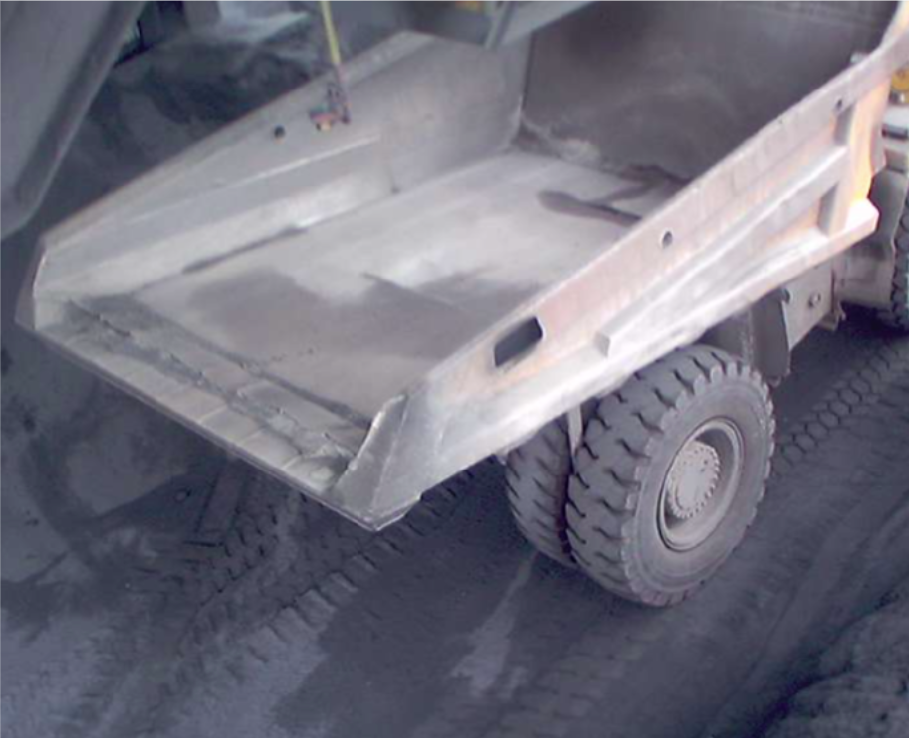
\includegraphics[width=\linewidth]{./Figuras/suciedad_a.png}
    \caption{Lente en óptimas condiciones.}
    \label{subfig:parte_a}
  \end{subfigure}
  \hfill
  \begin{subfigure}[b]{0.48\textwidth}
    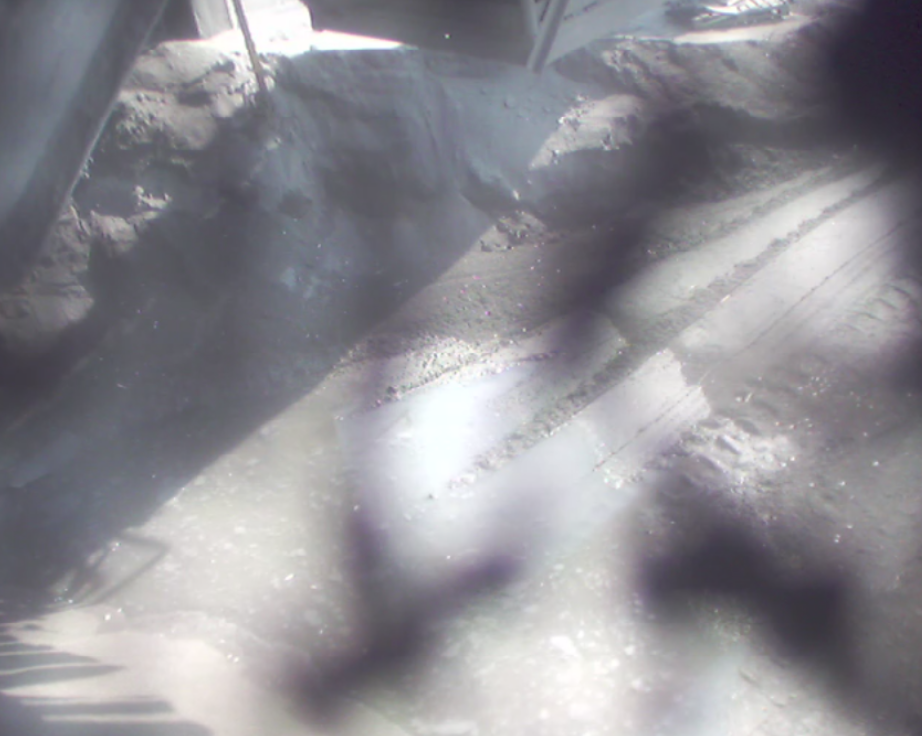
\includegraphics[width=\linewidth]{./Figuras/suciedad_b.png}
    \caption{Lente en malas condiciones.}
    \label{subfig:parte_b}
  \end{subfigure}
  \caption{Problema de suciedad en lentes que pueden presentar las cámaras, debido al entorno en el que se encuentran.}
  \label{fig:ej_suciedad}
\end{figure}

Esta problemática da lugar a la necesidad de desarrollar un sistema que permita conocer el estado actual de las principales cámaras de la empresa. Al tener información precisa sobre las condiciones en las que se encuentran, los resultados de los algoritmos de visión artificial van a ser los esperados y se pueden planificar las rondas de mantenimiento solo en caso de ser necesarias. 

Como se puede observar en el diagrama de la figura \ref{fig:diagrama_solucion}, la implementación del sistema requiere la configuración de los servicios necesarios para mantener el contenedor y la base de datos SQL Server a utilizar. El contenedor desplegado en las instalaciones locales (on-premises) accederá a todas las cámaras necesarias y analizará los problemas mencionados, registrando el estado actual en una tabla y generando las alarmas configuradas. Posteriormente, cada sector interesado podrá desarrollar los tableros necesarios para visualizar las cámaras de su interés. Las herramientas principales para crear las visualizaciones serán PIMS de AVEVA y PowerBI de Microsoft.

\begin{figure}[htpb]
\centering 
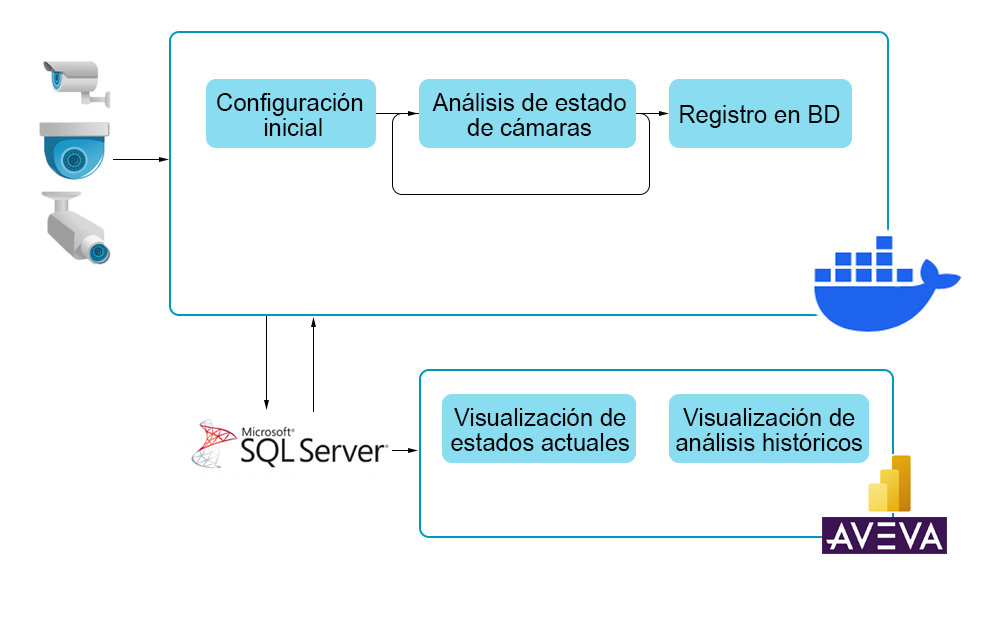
\includegraphics[width=.95\textwidth]{./Figuras/diagrama_inicial.png}
\caption{Diagrama en bloques del sistema.}
\label{fig:diagrama_solucion}
\end{figure}

\section{2. Identificación y análisis de los interesados} %listo v1
\label{sec:interesados}

\begin{table}[ht]
%\caption{Identificación de los interesados}
%\label{tab:interesados}
\begin{tabularx}{\linewidth}{@{}|l|X|X|l|@{}}
\hline
\rowcolor[HTML]{C0C0C0} 
Rol           & Nombre y Apellido & Organización & Puesto \\ \hline
Cliente       & \clientename  &\empclientename & Ger. Área Innov. \& Des.\\ \hline
Responsable   & \authorname  & FIUBA  & Alumno 	\\ \hline
Colaboradores & Pablo Rufach &\empclientename & BP Innovación  \\ \hline
Orientador    & \supname	&\pertesupname & Director del Trabajo Final \\ \hline
Usuario final & - & Prosegur y \empclientename & - \\ \hline
\end{tabularx}
\end{table}

\begin{itemize}
	\item Colaboradores: Pablo Rufach experto en infraestructura colaborará con el despliegue de los servicios necesarios y puesta en marcha de los servidores.
	\item Usuario final: personal de Prosegur encargado de la video vigilancia y equipo de mantenimiento perteneciente a \empclientename .
\end{itemize}

\section{3. Propósito del proyecto}
\label{sec:proposito}

Continuando con la estrategia de optimización de recursos implementada por \empclientename, el objetivo es establecer un sistema de monitoreo para evaluar el estado y detectar posibles problemas en las cámaras de manera proactiva. Se espera lograr un ahorro significativo al identificar y abordar los problemas de las cámaras antes de que afecten negativamente a las operaciones productivas. Además, este enfoque permitirá una toma de decisiones más informada en lo que respecta al mantenimiento preventivo, contribuyendo así a la reducción de costos y al aumento de la disponibilidad y fiabilidad de los sistemas.

\section{4. Alcance del proyecto}
\label{sec:alcance}

El proyecto abarcará los siguientes puntos y etapas:

\begin{itemize}
	\item Investigación de métodos y técnicas de VA para la detección y estimación de los problemas que se pueden presentar en las cámaras, listados en la sección \ref{sec:descripcion}.
	\item Implementación en las cámaras más relevantes de los algoritmos de Visión Artificial investigados, garantizando que satisfagan los requisitos establecidos. 
	\item Desarrollo del algoritmo para la toma de decisiones que generará las alertas.
	\item Definición de la estructura y creación de la base de datos utilizando SQL Server.
	\item Despliegue de la solución, mediante la utilización de contenedores, en el datacenter de \empclientename .
\end{itemize}

Puntos no comprendidos en el proyecto:

\begin{itemize}
	\item Diseño y desarrollo de una interfaz de usuario para facilitar la configuración del sistema.
	\item Incorporación de las visualizaciones especificadas en la figura \ref{fig:diagrama_solucion}.
	\item Mejora del rendimiento, con el objetivo de lograr velocidades óptimas en la detección y estimación.
\end{itemize}


\section{5. Supuestos del proyecto}
\label{sec:supuestos}

Para el desarrollo del presente proyecto se supone que:

\begin{itemize}
	\item Se contará con el tiempo suficiente para la realización del proyecto a pesar de las obligaciones personales, académicas y laborales.
	\item Existen métodos y técnicas de visión artificial que permitan obtener los resultados esperados.
	\item Se tendrá disponibilidad de los equipos necesarios para el desarrollo e implementación del sistema, destacando la necesidad de un servidor en condiciones y una notebook con GPU.
	\item La gerencia de infraestructura de \empclientename \ otorgará el acceso al servidor y las cámaras dentro de los plazos establecidos.
	\item Se cuenta con una conectividad confiable y estable entre el servidor y las cámaras a utilizar.
	\item Los usuarios finales contarán con el tiempo necesario para recibir las capacitaciones requeridas.
\end{itemize}

\section{6. Requerimientos}
\label{sec:requerimientos}

\begin{enumerate}
	\item Requerimientos funcionales:
		\begin{enumerate}
			\item El sistema debe permitir al usuario seleccionar los análisis a realizar para cada cámara integrada.
			\item Se requiere estimar los grados de rotación experimentados por la cámara durante el intervalo de tiempo configurado, además de detectar la suciedad en sus lentes ópticos.
			\item Debe ser capaz de generar alertas cuando las condiciones de las cámaras no cumplan con los parámetros definidos inicialmente.
			\item El sistema debe generar registros de las detecciones realizadas.
			\item Se necesitan realizar análisis periódicos de las cámaras configuradas.
			\item Se debe registrar el tiempo de inicio y finalización de cada alarma generada.
		\end{enumerate}
	\item Requerimientos durante el desarrollo/diseño:
		\begin{enumerate}
			\item El código debe ser desarrollado utilizando control de versiones con Git.
			\item Se debe garantizar la escalabilidad del sistema en términos de cantidad de cámaras y tipos de detecciones.
			\item Se deberá seleccionar el método de análisis que utilice la menor cantidad de recursos, siempre y cuando cumpla con los requerimientos funcionales.
			\item Se prefiere que el código sea desarrollado en Python.
			\item El diseño del sistema debe ser modular.
			\item El sistema debe implementarse en un ambiente on-premise.
			\item La base de datos generada por el sistema debe contener información sobre las cámaras, los resultados de los análisis, la configuración y los registros de estado interno del sistema.
		\end{enumerate}
	\item Requerimientos de documentación:
		\begin{enumerate}
			\item Se debe generar un manual de usuario que incluya los pasos a seguir frente a las alertas generadas por el sistema.
		\end{enumerate}
	\item Requerimientos de prueba y validación:
		\begin{enumerate}
			\item El sistema debe lograr una precisión superior al 90\% en la generación de alarmas.
			\item Se deben realizar pruebas del sistema en un entorno industrial para validar su confiabilidad.
		\end{enumerate}
	\item Requerimiento de seguridad de la información:
		\begin{enumerate}
			\item El sistema no debe permitir a los usuarios acceder a la visualización directa de las cámaras. La visualización debe realizarse únicamente a través del sistema de CCTV centralizado de \empclientename.
			\item El acceso a la información generada por el sistema debe estar restringido y protegido adecuadamente.
		\end{enumerate}
\end{enumerate}

\section{7. Historias de usuarios (\textit{Product backlog})}
\label{sec:backlog}

Para comenzar, se identifican los roles de las personas involucradas con un mayor detalle:

\begin{itemize}
	\item Gerente área innovación \& desarrollo: Responsable de la supervisión y dirección estratégica de proyectos de innovación tecnológica en la empresa.
	\item Ingeniero de mantenimiento: Encargado de garantizar el funcionamiento óptimo de las cámaras de vigilancia y de implementar medidas preventivas y correctivas.
	\item Técnico de mantenimiento: Apoya al ingeniero de mantenimiento en la ejecución de tareas diarias de inspección y mantenimiento de las cámaras.
	\item Gerente de seguridad: Encargado de supervisar y asegurar la integridad y confidencialidad de los sistemas de seguridad y vigilancia.
	\item Técnico operador de Prosegur: Personal encargado de la operación y monitoreo diario de las cámaras de seguridad.
	\item Analista de Datos: Profesional encargado de analizar los datos generados por el sistema y diseñar visualizaciones efectivas para comunicar la información de manera clara y comprensible.
\end{itemize}

A continuación, se presentan las historias de usuario, ponderadas según los siguientes criterios: tiempo requerido, complejidad e incertidumbre. A cada uno se le asigna un puntaje, de acuerdo a la secuencia de Fibonacci, en el rango de 1 (bajo) a 5 (alto). Los \textit{story points} se calculan como el inmediato superior a la suma de los aspectos individuales dentro de la serie.

\begin{enumerate}
	\item Como técnico de mantenimiento, necesito que el sistema pueda estimar la rotación de las cámaras y detectar suciedad en sus lentes, para detectar posibles manipulaciones indebidas y garantizar la integridad de las imágenes capturadas.

\textit{Story points}: 13 (tiempo requerido: 5, complejidad: 5, incertidumbre: 3)	

	\item Como gerente del área de innovación \& desarrollo, deseo que los algoritmos desarrollados consuman los menos recursos posibles, para minimizar la inversión en servidores y su posterior mantenimiento. 
	
\textit{Story points}: 13 (tiempo requerido: 3, complejidad: 3, incertidumbre: 3)	

	\item Como gerente de seguridad, necesito que el sistema garantice la confidencialidad y restricción del acceso a la información generada, para proteger la privacidad de las imágenes y los datos capturados por las cámaras de vigilancia.
	
\textit{Story points}: 8 (tiempo requerido: 2, complejidad: 3, incertidumbre: 2)	

	\item Como gerente de seguridad, deseo recibir alertas cuando las cámaras no se encuentren en condiciones óptimas, para tomar acciones preventivas y garantizar la continuidad de la vigilancia en la planta.
	
\textit{Story points}: 5 (tiempo requerido: 1, complejidad: 1, incertidumbre: 2)	
	
	\item Como técnico operador de Prosegur, deseo un manual que explique los pasos a seguir frente a las alertas generadas por el sistema, para poder responder eficazmente a situaciones de riesgo o anomalías en las cámaras.
	
\textit{Story points}: 5 (tiempo requerido: 2, complejidad: 2, incertidumbre: 1)			
	\item Como analista de datos, deseo tener toda la información necesaria centralizada en una única base de datos, para facilitar el desarrollo de las visualizaciones necesarias por los usuarios finales.
	
\textit{Story points}: 3 (tiempo requerido: 1, complejidad: 1, incertidumbre: 1)			
	
	\item Como técnico de mantenimiento, quiero poder seleccionar los análisis a realizar para cada cámara, para personalizar la evaluación según las necesidades específicas de cada área de la empresa.
	
\textit{Story points}: 3 (tiempo requerido: 1, complejidad: 1, incertidumbre: 1)		
	
	\item Como ingeniero de mantenimiento, necesito tener la trazabilidad del estado de las cámaras, para poder evaluar el desempeño de los técnicos y poder identificar las zonas más problemáticas.
	
\textit{Story points}: 3 (tiempo requerido: 1, complejidad: 1, incertidumbre: 1)		
	
\end{enumerate}


\section{8. Entregables principales del proyecto}
\label{sec:entregables}

Los entregables del proyecto son:

\begin{itemize}
	\item Documentación sobre los datos almacenados y la estructura de la base de datos.
	\item Código fuente del software.
	\item Diagramas sobre el funcionamiento del sistema.
	\item Memoria del trabajo final.
\end{itemize}

\section{9. Desglose del trabajo en tareas}
\label{sec:wbs}

\begin{enumerate}
\item Planificación (50 h)
	\begin{enumerate}
	\item Reuniones con el personal involucrado en el proyecto. (10 h)
	\item Análisis de alcance y requerimientos. (10 h)
	\item Realizar el plan del proyecto. (30 h)
	\end{enumerate}
\item Investigación preliminar (110 h)
	\begin{enumerate}
	\item Explorar proyectos relacionados y mejores prácticas. (20 h)
	\item Investigar modelos pre-entrenados. (20 h)
	\item Investigar algoritmos de visión artificial. (30 h) 
	\item Estudiar las herramientas y tecnologías para la implementación. (20 h)
	\item Evaluar los requisitos de seguridad. (20 h)
	\end{enumerate}
\item Diseño y desarrollo (285 h)
	\begin{enumerate}
	\item Diseñar la arquitectura del sistema. (20 h)
	\item Crear la estructura de la base de datos e implementarla. (10 h)
	\item Desarrollar la estimación del angulo de rotación. (40 h)
	\item Desarrollar la detección de la suciedad en el lente óptico. (40 h)
	\item Desarrollar la detección de obstrucciones total o parciales. (40 h)
	\item Diseñar el sistema de alarmas. (25 h)
	\item Pruebas de integración y validación. (40 h)
	\item Dockerizar la solución desarrollada. (40 h)
	\item Optimización y búsqueda de errores. (30 h)
	\end{enumerate}
\item Implementación y capacitaciones (115 h)
	\begin{enumerate}
	\item Preparar el servidor a utilizar y los servicios necesarios. (40 h)
	\item Crear los pipeline y configuraciones necesarias para el despliegue. (30 h)
	\item Implementar la solución. (30 h)
	\item Preparación de materiales de capacitación. (5 h)
	\item Organizar y Realizar sesiones de capacitación. (10 h)
	\end{enumerate}
\item Documentos finales (105 h)
	\begin{enumerate}
	\item Redacción de la documentación sobre los datos almacenados y la estructura de la base de datos. (5 h)
	\item Elaboración de diagramas sobre el funcionamiento del sistema. (5 h)
	\item Confección de informe de avance. (15 h)
	\item Redacción de memoria del trabajo. (60 h)
	\item Elaboración de la presentación final. (20 h)
	\end{enumerate}
\end{enumerate}

Cantidad total de horas: 665 h.

\end{document}